% IEEE conference version for GTSD 2026 proceedings
\documentclass[conference]{IEEEtran}
\usepackage{cite}
\usepackage{amsmath,amssymb,amsfonts}
\usepackage{graphicx}
\graphicspath{{figures/}}
\usepackage{textcomp}
\usepackage{booktabs}
\usepackage{url}
\def\BibTeX{{\rm B\kern-.05em{\sc i\kern-.025em b}\kern-.08em
    T\kern-.1667em\lower.7ex\hbox{E}\kern-.125emX}}

\begin{document}
\bstctlcite{IEEEexample:BSTcontrol}

\section{Related Work}

\subsection{Deep Learning Paradigms for Single Image Super-Resolution}

Over the past decade, deep learning architectures for Single Image Super-Resolution (SISR) have undergone substantial evolution, which can be categorized primarily by the spatial positioning of their upsampling operations: \textit{pre-upsampling} and \textit{post-upsampling} frameworks \cite{yang2019deep, liu2025comprehensive}. 

In early pre-upsampling architectures, exemplified by SRCNN \cite{dong2014learning} and VDSR \cite{kim2016accurate}, the Low-Resolution (LR) input image is first interpolated to the target High-Resolution (HR) spatial grid using traditional bicubic interpolation before entering the neural network. Consequently, the convolutional layers operate solely as a non-linear mapping engine dedicated to reconstructing lost high-frequency spatial components. Because all hidden layers maintain a uniform spatial resolution throughout the network pipeline, pre-upsampling models establish a highly regular, strictly feed-forward streaming dataflow. From a hardware design perspective, this dimensional uniformity eliminates multi-rate clock domain crossings and complex spatial re-indexing, thereby substantially simplifying streaming on-chip line buffer and pipelined compute architectures. Conversely, post-upsampling frameworks, pioneered by FSRCNN \cite{dong2016accelerating} and ESPCN \cite{shi2016real}, perform feature extraction directly within the compact LR coordinate space and defer spatial magnification to the final stage via transposed convolution (deconvolution) or sub-pixel convolution (PixelShuffle). Although this design reduces theoretical floating-point operations (FLOPs) on general-purpose processors, it introduces significant structural irregularities into streaming Register-Transfer Level (RTL) pipelines. Fig.~\ref{fig:sr_paradigms} illustrates this structural distinction across the three representative architectures.

\begin{figure}[t]
\centering
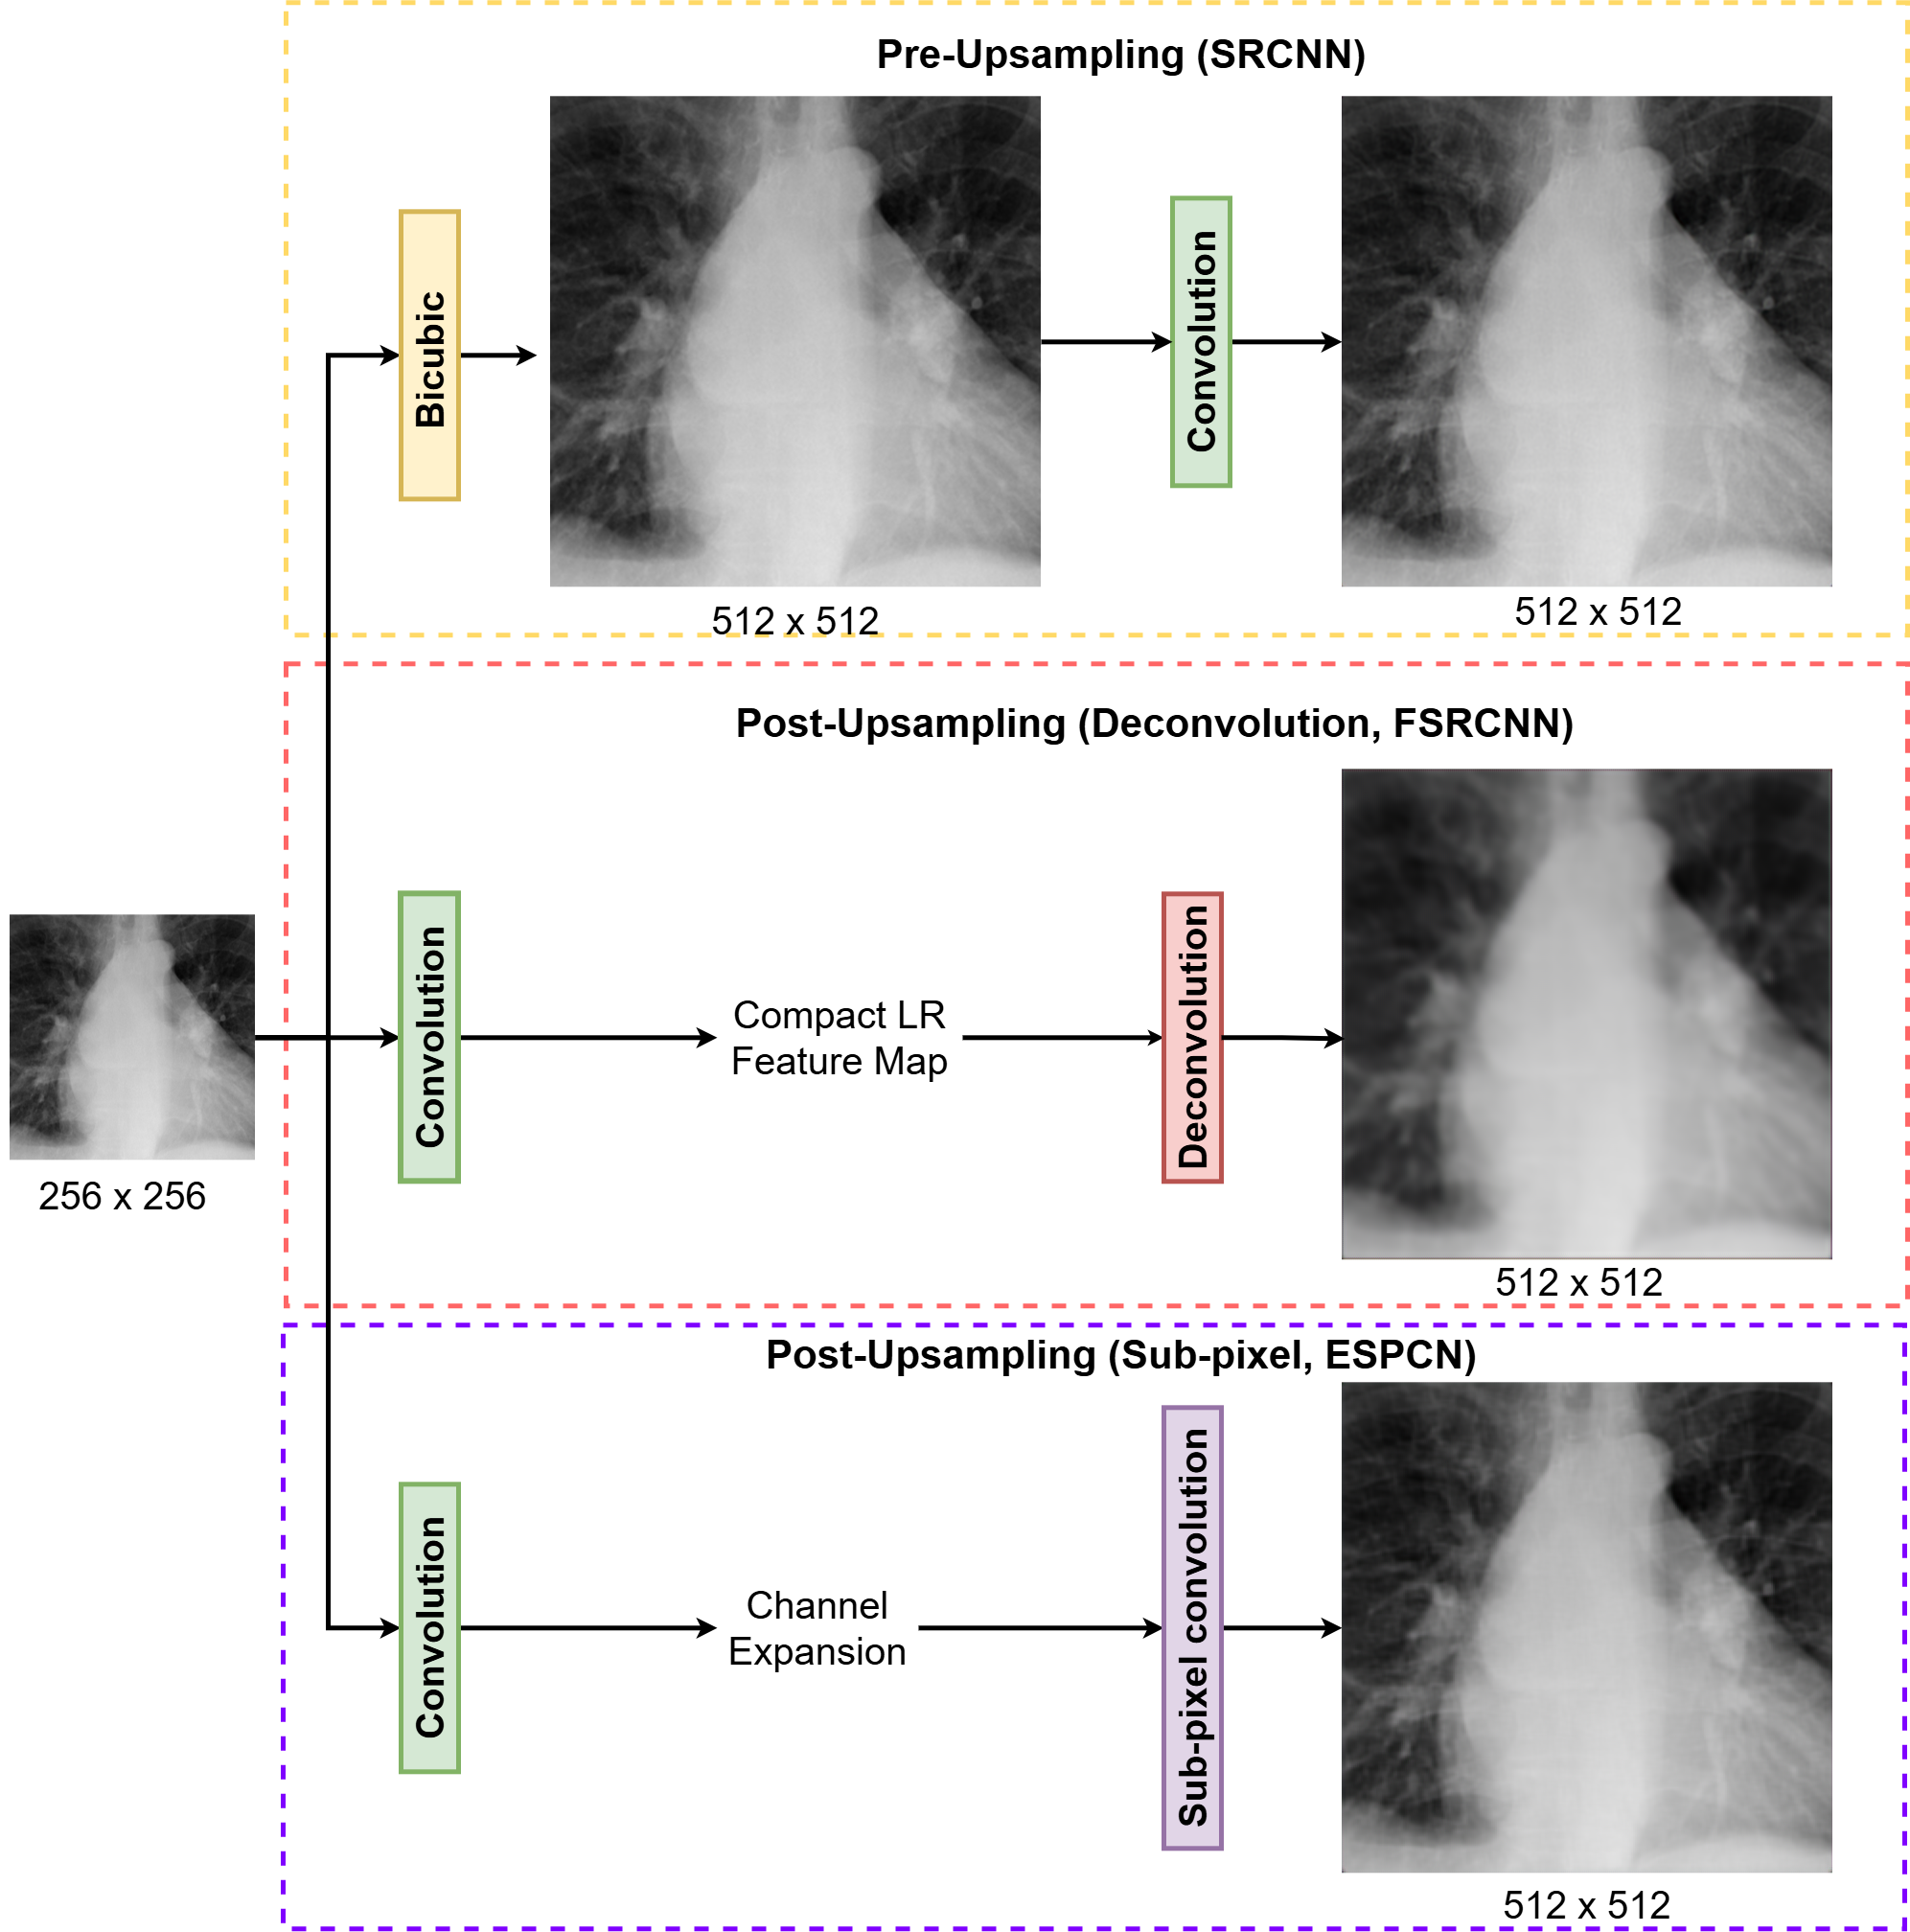
\includegraphics[width=\columnwidth]{upsample_methods_2x.png}
\caption{Comparison of pre-upsampling (SRCNN) and post-upsampling (FSRCNN via deconvolution; ESPCN via sub-pixel convolution) super-resolution pipelines on a $256 \times 256$ chest radiograph upscaled to $512 \times 512$ ($\times 2$). The deconvolution-based output exhibits visible blurring and structural degradation consistent with the checkerboard-artifact mechanism discussed in Section~II-A.}
\label{fig:sr_paradigms}
\end{figure}

For safety-critical, resource-constrained medical edge deployments, post-upsampling and generative reconstruction models present severe hardware and clinical limitations. Specifically, transposed convolution layers rely on an interleaved zero-insertion pattern across their activation or weight matrices, which leads to idle Multiply-Accumulate (MAC) cycles and non-contiguous memory access patterns on hardware. More critically, uneven filter overlap during transposed convolution is a well-established source of periodic grid-like artifacts, commonly referred to as \textit{checkerboard artifacts} \cite{odena2016deconvolution}. As visually demonstrated in Fig.~\ref{fig:sr_paradigms}, the deconvolution-based reconstruction exhibits noticeably coarser, blockier structure compared to the pre-upsampling and sub-pixel approaches, consistent with the checkerboard-artifact mechanism described by Odena \textit{et al.} \cite{odena2016deconvolution}. In diagnostic medical imaging, checkerboard artifacts represent an unacceptable clinical hazard rather than a mere aesthetic degradation: periodic high-frequency grid distortions can visually obscure subtle anatomical margins or masquerade as pathological micro-lesions, fine tissue infiltrates, or calcifications. 

While sub-pixel convolution (PixelShuffle) eliminates deconvolutional checkerboard artifacts and reduces theoretical arithmetic operations by operating on the low-resolution grid, it introduces substantial control and memory overhead into streaming Register-Transfer Level (RTL) pipelines. Specifically, PixelShuffle mandates complex multi-phase channel demultiplexing, multi-bank memory shuffling, and asynchronous multi-rate clock domain crossings between the Low-Resolution feature extraction core and the High-Resolution output interface. For deep, compute-heavy networks comprising dozens of cascading layers (such as RCAN or EDSR), the $r^2$ arithmetic reduction easily justifies this architectural overhead. Conversely, for an ultra-compact three-layer mapping network like SRCNN ($\approx 69\text{k}$ parameters), the absolute computational volume is already negligible ($<0.09$~GMACs per patch). In this lightweight regime, the hardware area, routing congestion, and latency penalty of spatial re-ordering logic far outweigh any arithmetic power savings. By combining a single-rate streaming bicubic pre-interpolator with dimensionally uniform convolution stages, our pre-upsampling pipeline guarantees 100\% Multiply-Accumulate (MAC) efficiency (one output pixel per clock cycle) with strictly feed-forward line buffering and zero pipeline stall overhead.

Similarly, while Generative Adversarial Networks (GANs) such as SRGAN \cite{ledig2017photo} and ESRGAN \cite{wang2018esrgan} synthesize visually sharp, photorealistic textures via adversarial and perceptual objectives, they do not reconstruct the true deterministic underlying radiological signal. Instead, generative priors synthesize plausible synthetic details, introducing an inherent risk of structural hallucinations \cite{bhadra2021hallucinations, giraldo2024perceptual}. Furthermore, deep generative architectures such as SRGAN \cite{ledig2017photo} (which constructs a 16-residual-block generator with deep multi-stage feature cascades) and ESRGAN \cite{wang2018esrgan} require large model capacities and deep hierarchical convolutions that far exceed the on-chip Block RAM and 220 DSP48E1 slice budget of edge-class SoCs. Therefore, given (a) strict dataflow regularity, (b) complete avoidance of deconvolution-induced checkerboard artifacts, (c) elimination of PixelShuffle memory-reordering overhead, and (d) elimination of generative hallucination risks, a compact pre-upsampling mapping-based CNN (SRCNN) represents the most clinically defensible and hardware-amenable choice for edge medical radiography.

\subsection{FPGA-Based Hardware Accelerators for CNNs}

Accelerating deep convolutional networks on Field-Programmable Gate Arrays (FPGAs) has garnered widespread interest due to their deterministic latency, fine-grained reconfigurability, and competitive energy efficiency \cite{sze2017efficient, mittal2020survey}. Convolutional operations are fundamentally memory-intensive; repeatedly fetching overlapping $K \times K$ receptive fields from off-chip dynamic RAM (DRAM) quickly saturates external memory bandwidth, causing severe throughput degradation known as the ``memory wall'' \cite{sze2017efficient}. To resolve this bottleneck, state-of-the-art RTL accelerators employ 2D line-buffer topologies composed of on-chip Block RAMs (BRAMs) and cascading shift-registers. A line buffer caches only $K-1$ rows of pixels on-chip, enabling single-port streaming data ingestion while simultaneously feeding a complete $K \times K$ spatial kernel to the compute core on every clock cycle. Concurrently, a parallel MAC array paired with a balanced, pipelined adder reduction tree processes all $K^2$ multiplications and summations concurrently, achieving an optimal computational throughput of one output pixel per clock cycle without stalling \cite{sze2017efficient, mittal2020survey}.

\begin{table*}[t]
\centering
\caption{Comparison of FPGA-Based Super-Resolution Accelerators}
\label{tab:fpga_comparison}
\renewcommand{\arraystretch}{1.3}
\setlength{\tabcolsep}{5pt}
\resizebox{\textwidth}{!}{%
\begin{tabular}{lcccccc}
\hline
\textbf{Work} & \textbf{Target Platform} & \textbf{DSPs Used} & \textbf{Full-Chip Power} & \textbf{Throughput / Latency} & \textbf{Precision} & \textbf{Application / Model} \\
\hline
Mao \textit{et al.} \cite{mao2020fdna} (2020) & Xilinx FPGA & 1512 & 5.40 W & 62.7 fps (UHD) & Fixed 13-bit & Natural Images / F-DNA (FSRCNN) \\
Liu \textit{et al.} \cite{liu2024high} (2024) & Xilinx FPGA & 1210 & 16.85 W & 35.8 fps (FHD) & Fixed 8-bit & Natural Images / Edge SR \\
Chang \textit{et al.} \cite{chang2024hdsuper} (2024) & Xilinx FPGA & 704 & 2.08 W & 81.0 fps (FHD) & Fixed 16-bit & Natural Images / HDSuper (LSR) \\
Huang \textit{et al.} \cite{huang2026uasr} (2026) & Xilinx ZCU102 & 181 (7.2\%) & 2.88 W & 83.0 fps (FHD) & Fixed 16-bit & Natural Images / UASR-A \\
\hline
\textbf{This Work} & \textbf{Xilinx Zynq-7020} & \textbf{120 (54.5\%)} & \textbf{1.438 W} & \textbf{157.9 patches/s} & \textbf{PTQ Q7 (INT8)} & \textbf{Medical X-Ray / SRCNN} \\
 & (PYNQ-Z2 Edge SoC) & (PL Dynamic: 0.047 W) & (Full-Chip Total) & (6.33 ms/patch) & (S7.0 / S0.7) & (100 MHz Streaming RTL) \\
\hline
\end{tabular}%
}
\end{table*}

Despite these advancements, a critical resource and thermal gap remains in existing FPGA-based SR acceleration literature. Recent notable contributions, such as the deconvolutional acceleration engine F-DNA by Mao \textit{et al.} \cite{mao2020fdna}, the real-time edge accelerator by Liu \textit{et al.} \cite{liu2024high}, the lightweight co-design accelerator HDSuper by Chang \textit{et al.} \cite{chang2024hdsuper}, and the edge attention accelerator UASR-A by Huang \textit{et al.} \cite{huang2026uasr}, have demonstrated commendable reconstruction throughput. However, as benchmarked in Table~\ref{tab:fpga_comparison}, these accelerators primarily target high-tier or mid-range FPGA platforms (e.g., ZCU102 or large Virtex/Kintex devices) with expansive logic fabrics, consuming between 181 and 1512 DSP blocks and operating within a 2.08~W to 16.85~W thermal envelope. Such hardware resource footprints are fundamentally incompatible with entry-level, cost-sensitive edge devices (e.g., the low-cost Xilinx Zynq-7020 with only 220 total DSP slices) and strict sub-1.5~W full-chip power constraints required by portable bedside radiography and point-of-care medical modalities. Furthermore, existing accelerators exclusively evaluate natural photography benchmarks (such as Set5 and Set14), overlooking clinical diagnostic fidelity, boundary tiling discontinuities, and quantization-induced radiological feature preservation.

To bridge this research gap, our work demonstrates that a hardware-tailored 3-layer SRCNN with 8-bit Post-Training Quantization (PTQ Q7) implemented on an entry-level Xilinx Zynq-7020 SoC achieves high clinical reconstruction fidelity (39.28~dB PSNR, 0.9598 SSIM on Chest X-Ray radiography) while utilizing only 120 DSP48E1 slices (54.55\% of budget) and dissipating merely 1.438~W full-chip power (with an ultra-low PL dynamic power of 0.047~W).

% Page break to cleanly isolate standalone bibliography and avoid column bleeding
\newpage
\bibliographystyle{IEEEtran}
\bibliography{bib/references}
\end{document}